\renewcommand{\theequation}{\theenumi}
\begin{enumerate}[label=\arabic*.,ref=\thesubsection.\theenumi]
\numberwithin{equation}{enumi}
%\item If three  sides of one triangle are equal to three sides  of the other triangle, then the two triangles are congruent (SSS Congruence Rule).
%%
%\\
%\solution Using cosine formula in \eqref{eq:b_cos_form}, it can be shown that the angles of the triangle are also equal, hnce they are congruent.
% 	
%\item If two sides and the included angle of one triangle are equal to two sides and the included angle of the other triangle, then the two triangles are congruent (SAS Congruence Rule).
%\\
%\solution Use cosine formula in \eqref{eq:b_cos_form}.
%\item  If two angles and the included side of one triangle are equal to two angles and the included side of the other triangle, then the two triangles are congruent (ASA Congruence Rule).
%%
%\\
%\solution  Use the sine formula in \eqref{eq:sin_form} to show that the corresponding sides opposite the angles are equal. 
%\item If two angles and one side of one triangle are equal to two angles and the corresponding side of the other triangle, then the two triangles are congruent (AAS Congruence Rule)
%\\
%\solution Use the sine formula in \eqref{eq:sin_form}

%\item  In a triangle, angle opposite to the longer side is larger (greater). 
%%
%\label{prob:tri_ang_side_greater}
%%
%\\
%\solution Consider a right triangle $ABC$ right angled at $B$ as in Fig. \ref{fig:tri_ang_side_greater}.  From Baudhayana's theorem, 
%%
%\begin{align}
%\label{eq:tri_ang_side_greater_baudhb}
%b^2 &= a^2+c^2
%\\
%p^2 &= a^2+x^2
%\label{eq:tri_ang_side_greater_baudhp}
%\end{align}
%%
%$\because c > x$, from \eqref{eq:tri_ang_side_greater_baudhb} and \eqref{eq:tri_ang_side_greater_baudhp}, is obvious that %
%\begin{align}
%\label{eq:tri_ang_side_greater_baudhbp}
%b > p \implies \frac{b}{p} > 1
%\end{align}
%%
%Also, from \eqref{eq:sin_form_def},
%%
%%
%\begin{align}
%%\label{eq:tri_ang_side_greater_baudh_bp}
%a = b\sin A &= p \sin \theta 
%\implies \frac{b}{p} &= \frac{\sin \theta}{\sin A} > 1
%\\
%\text{or, } \sin \theta > \sin A
%\end{align}
%%
%from \eqref{eq:tri_ang_side_greater_baudhbp}.   Note that this is always true.  Thus, 
%%
%\begin{align}
%\label{eq:tri_ang_side_greater_final}
%\theta > A \iff \sin \theta > \sin A
%\end{align}
%%
%In any $\triangle ABC$,  using \eqref{eq:sin_form} and \eqref{eq:tri_ang_side_greater_final},
%
%%
%%
%\begin{align}
%a>b \implies \frac{a}{b} = \frac{\sin A}{\sin B} > 1 
%\\
%\text{or, }  \sin A > \sin B \implies A > B
%\end{align}
%%
%In any $\triangle ABC$, if $A>B$, using \eqref{eq:sin_form},
%%
%\begin{figure}[!ht]
%\includegraphics[width=\columnwidth]{./triangle/figs/tri_ang_side_greater.eps}
%\caption{}
%\label{fig:tri_ang_side_greater}
%\end{figure}
%

%\item In a triangle, side opposite to the larger (greater) angle is longer. 
%%
%\\
%\solution Use \eqref{eq:sin_form} and \eqref{eq:tri_ang_side_greater_final}.
%
\item Do the points $\vec{A}=\myvec{3\\2}, \vec{B}=\myvec{-2\\-3}, \vec{C}=\myvec{2\\3} $ form a triangle?  If so, name the type of triangle formed.
\label{prob:tri_exam_coll_pts}
%
\\
\solution The direction vectors of $AB$ and $BC$ are 
\begin{align}
\label{eq:tri_geo_ex_baorth}
\vec{B}-\vec{A} &= \myvec{-5\\-5}
\\
\vec{C}-\vec{A} &= \myvec{-1\\1}
\label{eq:tri_geo_ex_caorth}
\end{align}
%
Since 
%
\begin{align}
\vec{B}-\vec{A} \ne k\brak{\vec{C}-\vec{A}},
\end{align}
%
the points are not collinear and form a triangle.  An alternative method is to create the matrix
\begin{align}
\label{eq:tri_geo_ex_diff_mat}
\vec{M} = \myvec{\vec{B}-\vec{A} & \vec{B}-\vec{A}}^T 
\end{align}
%
If $rank(\vec{M}) = 1$, the points are collinear.  The rank of a matrix is the number of nonzero rows left after doing row operations.  In this problem, 
%
\begin{align}
\vec{M} = \myvec{-5 & -5\\-1 & 1}\xleftrightarrow {R_2\leftarrow 5R_2-R_1}\myvec{-5 & -5\\0 & 10}
\\
\implies rank(\vec{M}) = 2
\end{align}
%
as the number of non zero rows is 2.
The following code plots Fig. \ref{fig:check_tri}
%
\begin{lstlisting}
codes/triangle/check_tri.py
\end{lstlisting}
%
\begin{figure}[!ht]
\includegraphics[width=\columnwidth]{./triangle/figs/check_tri.eps}
\caption{}
\label{fig:check_tri}
\end{figure}
%
From the figure, it appears that $\triangle ABC$ is right angled, with $BC$ as the hypotenuse.  From Baudhayana's theorem, this would be true if 
\begin{align}
\norm{\vec{B}-\vec{A}}^2+\norm{\vec{C}-\vec{A}}^2&=\norm{\vec{B}-\vec{C}}^2
\end{align}
which, from \eqref{eq:tri_const_norm_ac} can be expressed as
\begin{multline}
\norm{\vec{A}}^2 + \norm{\vec{C}}^2 - 2\vec{A}^T\vec{C}+
\norm{\vec{A}}^2 + \norm{\vec{B}}^2 - 2\vec{A}^T\vec{B}
\\
=
\norm{\vec{B}}^2 + \norm{\vec{C}}^2 - 2\vec{B}^T\vec{C}
\end{multline}
%
to obtain 
\begin{align}
\label{eq:tri_geo_ex_orth}
\brak{\vec{B}-\vec{A}}^T\brak{\vec{C}-\vec{A}}&=0
\end{align}
%
after simplification.  From \eqref{eq:tri_geo_ex_baorth} and \eqref{eq:tri_geo_ex_caorth}, it is easy to verify that 
\begin{align}
\label{eq:tri_geo_ex_orth_sol}
\brak{\vec{B}-\vec{A}}^T\brak{\vec{C}-\vec{A}}=
 \myvec{-5 & -5}\myvec{-1\\1} = 0
\end{align}
satisfying
\eqref{eq:tri_geo_ex_orth}. Thus,  $\triangle ABC$ is right angled at $\vec{A}$.
%
%
%\item Area of a triangle is half the product of its base and the corresponding altitude. 
%%
%\\
%\solution First, we consider the right angled triangle in Fig\ref{fig:tri_right_area}. By definition, the area of the rectangle $ABCD$ is $ac$.  Also, The rectangle is a sum of two congruent triangles $ABC$ and $ADC$.  Thus,
%%
%\begin{align}
%\text{ar}\triangle ABC=\text{ar}\triangle ADC = \frac{1}{2}ac
%\end{align} 
%%
%\begin{figure}[!ht]
%\includegraphics[width=\columnwidth]{./triangle/figs/tri_right_area.eps}
%\caption{}
%\label{fig:tri_right_area}
%\end{figure}
%%
%For any $\triangle ABC$, as shown in Fig.  \ref{fig:tri_area}, the area can be obtained as
%%
%\begin{align}
%\text{ar}\triangle ABC&=\frac{1}{2}xh+\frac{1}{2}yh 
%\\
%\frac{1}{2}\brak{x+y}h = \frac{1}{2}ah
%\end{align} 
%%

%
%\begin{figure}[!ht]
%\includegraphics[width=\columnwidth]{./triangle/figs/tri_area.eps}
%\caption{}
%\label{fig:tri_area}
%\end{figure}
%
\item Find the area of a triangle whose vertices are 
$\vec{A}=\myvec{1\\-1}, 
\vec{B} = \myvec{-4\\6}$ and
$ 
\vec{C} = \myvec{-3\\-5}
$.
%
\\
\solution
  Using Hero's formula, the following code computes the area of the  triangle as 24.
%
\begin{lstlisting}
codes/triangle/area_tri.py
\end{lstlisting}
%
%\item A median of a triangle divides it into two triangles of equal areas.
%\\
%\solution In $\triangle ABC$, let $AD$
%
\item Find the area of a triangle formed by the vertices $\vec{A}=\myvec{5\\2}, \vec{B}=\myvec{4\\7}, \vec{C}=\myvec{7\\-4}$.
%\\
\solution  The area of $\triangle ABC$ is also obtained  in terms of the  {\em magnitude} of the determinant of the matrix $\vec{M}$ in  \eqref{eq:tri_geo_ex_diff_mat} as
%
\begin{align}
\frac{1}{2}\mydet{\vec{M}}
\end{align}
The computation is done in \textbf{area\_tri.py}
\item Find the area of a triangle formed by the points $\vec{P}=\myvec{-1.5\\3}, \vec{Q}=\myvec{6\\-2}, \vec{R}=\myvec{-3\\4}$.
\\
\solution Another formula for the area of $\triangle ABC$  is
%
\begin{align}
\frac{1}{2}\mydet{1 & 1 & 1\\ \vec{A} & \vec{B} & \vec{C} }
\end{align}
%
\item Find the area of a triangle having the points
%
\begin{align}
\vec{A} = \myvec{1\\1 \\1},
\vec{B} = \myvec{1\\2 \\3},
\vec{C} = \myvec{2\\ 3\\1}
\end{align}
%
as its vertices.
\\
\solution The area of a triangle using the {\em vector product} is obtained as
\begin{align}
\frac{1}{2}\norm{\brak{\vec{B}-\vec{A}}\times \brak{\vec{C}-\vec{A}}}
\end{align}
%
For any two vectors $\vec{a}=\myvec{a_1\\a_2\\a_3}, \vec{b}=\myvec{b_1\\b_2\\b_3}$, 
\begin{align}
\label{eq:tri_cross_prod}
\vec{a}\times \vec{b} = \myvec{0 & -a_3 & a_2 \\ a_3 & 0 & -a_1 \\ -a_2 & a_1 & 0}\myvec{b_1\\b_2\\b_3}
\end{align}
%
The following code computes the area using the vector product.
%
\begin{lstlisting}
codes/triangle/area_tri_vec.py
\end{lstlisting}
%
%
\item The centroid of a $\triangle ABC$ is at the point \myvec{1\\1\\1}.  If the coordinates of $\vec{A}$ and $\vec{B}$ are \myvec{3\\-5\\7} and \myvec{-1\\7\\-6}, respectively, find the coordinates of the point $\vec{C}$.
%
\\
\solution The centroid of $\triangle ABC$ is given by
\begin{align}
\label{eq:tri_geo_ex_centroid}
\vec{O} = \frac{\vec{A}+\vec{B}+\vec{C}}{3}
\end{align}
%
Thus, 
\begin{align}
\vec{C} = 3\vec{C}-\vec{A}-\vec{B}
\end{align}
%
\item Show that the points 
\begin{align}
\vec{A} = \myvec{2\\-1 \\1},
\vec{B} = \myvec{1\\-3 \\-5},
\vec{C} = \myvec{3\\ -4\\-4}
\end{align}
%
are the vertices of a right angled triangle.
\\
\solution 
The following code plots Fig. \ref{fig:triangle_3d}
%
\begin{lstlisting}
codes/triangle/triangle_3d.py
\end{lstlisting}
%
\begin{figure}[!ht]
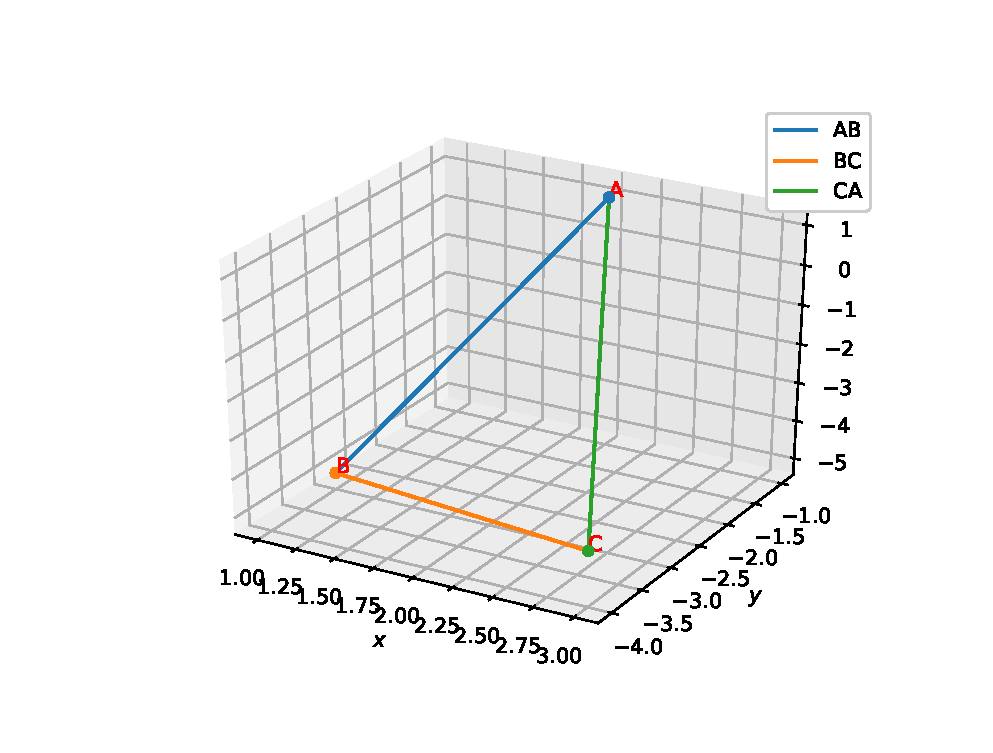
\includegraphics[width=\columnwidth]{./triangle/figs/triangle_3d.eps}
\caption{}
\label{fig:triangle_3d}
\end{figure}
%
From the figure, it appears that $\triangle ABC$ is right angled at $\vec{C}$.  Since 
\begin{align}
\brak{\vec{A}-\vec{C}}^T\brak{\vec{B}-\vec{C}}&=0
\end{align}
%
it is proved that the triangle is indeed right angled.
 \item Are the points 
\begin{align}
\vec{A} = \myvec{3\\6 \\9},
\vec{B} = \myvec{10\\20 \\30},
\vec{C} = \myvec{25\\ -41\\5},
\end{align}
%
the vertices of a right angled triangle?
%
%
\end{enumerate}
%
